\chapter{Overview}
\section{BAM}
BAM is Revature's batch management platform for recording and retrieving batch information. It is built with a cutting edge, micro service architecture to allow for modularity, system resilience, and fast development. It’s infrastructure services include a circuit breaking metric display, multiple discovery services for heartbeat monitoring, a configuration server for business service backups, and an API gateway that handles redirecting requests to different business services.

\section{Infrastructure}
\subsection{Discovery Service}
Discovery services are used to monitor business micro-services through the use of heart beats. This application utilizes Eureka to send heart beats out on timed intervals. This helps reduce API calls to micro-services that are no longer operational.

\subsection{Configuration Service}
Configuration Service used to apply a uniform configuration across specified micro-services. This application uses Configuration Server to provide configurations to any backup services that are needed to be spun up. It helps reduce repeated configuration files across micro-service applications.

\subsection{API Gateway}
API gateways are used to provide a single endpoint for client’s to access and it can apply filters across data. This application uses Zuul Netflix dependency to redirect client requests to different online business micro-services. It helps direct traffic throughout the system and allows for dynamic trafficking with the help of the circuit breaker.

\subsection{Circuit Breaking Service}
Circuit breaking is used to improve BAM’s resiliency. This application uses Hystrix dashboard and Hystrix circuit breaker to handle errors with fallback methods. The Hystrix dashboard allows easy monitoring of all business service clusters and their circuit breakers.

\subsection{Business Services}
Business services are the micro-services that handle any application specific operations. In BAM, these business services consist of: User micro-service, Batch micro-service, Curriculum micro-service, and Topic micro-service.Each of these micro-services persist data and also expose internal endpoints for any other business micro-service to request resources.

\subsection{Infrastructure Design}
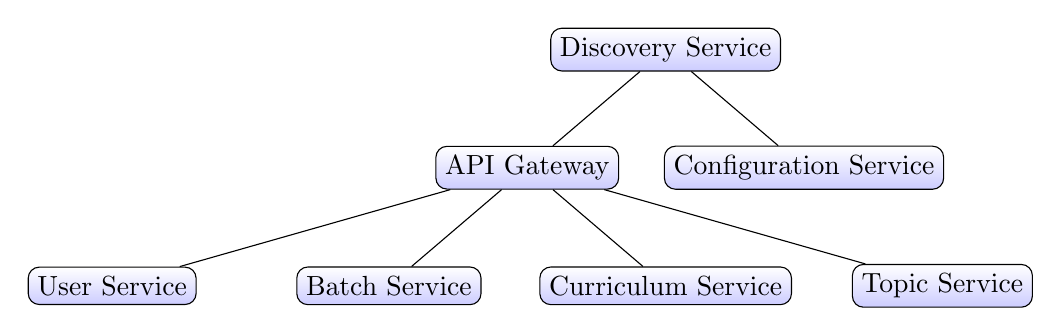
\begin{tikzpicture}[sibling distance=10em,
  every node/.style = {shape=rectangle, rounded corners,
    draw, align=center,
    top color=white, bottom color=blue!20}]]
  \node {Discovery Service}
    child { node {API Gateway}
        child { node {User Service}} 
        child { node {Batch Service}}
        child { node {Curriculum Service}}
        child { node {Topic Service}}}
    child { node {Configuration Service}};
\end{tikzpicture}
